\documentclass[11pt]{article}
\usepackage{fullpage}
\usepackage{amsmath}
\usepackage{amssymb}
\usepackage{amsthm}
\usepackage{mathabx}
\usepackage{color}
\usepackage{cancel}
\usepackage{wrapfig}
\usepackage{subcaption}
\usepackage{caption}
\usepackage{xfrac}
\usepackage{algorithm}
\usepackage{algorithmic}
\usepackage{mdframed}
\usepackage{hyperref}
\usepackage{xcolor}
\hypersetup{
	colorlinks,
	linkcolor={red!40!gray},
	citecolor={blue!40!gray},
	urlcolor={blue!70!gray}
}
\usepackage{cleveref}
\def\opt{{\textsc{OPT}_k}}
\def\const{{\mathrm{const}}}
\def\nnz{{\mathrm{nnz}}}
\def\r{\sfrac{\sigma_{\w}^2}{\sigma_{\xib}^2}}
\def\rm{\sfrac{\sigma_{\xib}^2}{\sigma_{\w}^2}}
\def\cmark{\Green{\checkmark}}
\def\xmark{\Red{\large\sffamily x}}
\newcommand{\pdet}{{\mathrm{pdet}}}
\newcommand{\MSPE}[1] {{\mathrm{MSPE}\big[#1\big]}}
\newcommand{\MSE}[1] {{\mathrm{MSE}\big[#1\big]}}
\def\Poisson{{\operatorname{Poisson}}}
\def\PB{{\operatorname{PB}}}
\newcommand{\DP}[1]{\mathcal{DP}^{#1}}
\def\Ic{\mathcal{I}}
\def\Jc{\mathcal{J}}
\def\Mc{\mathcal M}
\def\Ec{\mathcal E}
\def\sr{{\mathrm{sr}}}
\def\ktd{{k^{\underline{d}}}}
\def\Det{{\mathrm{Det}}}
\def\detu{{\widecheck{\mathrm{Det}}_\mu^\gamma}}
\def\deto{{\widehat{\mathrm{Det}}_\mu^\gamma}}
\def\Zu{{\widecheck{Z}_\mu^{\gamma}}}
\def\Zo{{\widehat{Z}_\mu^{\gamma}}}
\def\Zun{{\widecheck{Z}_\mu^{\gamma_n}}}
\def\Zon{{\widehat{Z}_\mu^{\gamma_n}}}
\newcommand{\Er}{\mathrm{Er}}
\newif\ifDRAFT
\DRAFTtrue
\ifDRAFT
\newcommand{\marrow}{\marginpar[\hfill$\longrightarrow$]{$\longleftarrow$}}
\newcommand{\niceremark}[3]
   {\textcolor{red}{\textsc{#1 #2:} \marrow\textsf{#3}}}
\newcommand{\ken}[2][says]{\niceremark{Ken}{#1}{#2}}
\newcommand{\manfred}[2][says]{\niceremark{Manfred}{#1}{#2}}
\newcommand{\michael}[2][says]{\niceremark{Michael}{#1}{#2}}
\newcommand{\michal}[2][says]{\niceremark{Michal}{#1}{#2}}
\newcommand{\feynman}[2][says]{\niceremark{Feynman}{#1}{#2}}
%\usepackage[inline]{showlabels}
\else
\newcommand{\ken}[1]{}
\newcommand{\michael}[1]{}
\newcommand{\michal}[1]{}
\newcommand{\feynman}[1]{}
\fi
\newcommand{\norm}[1]{{\| #1 \|}}

\newcommand{\deff}{d_{\textnormal{eff}}}
\def\ee{\mathrm{e}}
\newcommand\mydots{\makebox[1em][c]{.\hfil.\hfil.}}
\def\Sd{\mathscr{S}_{\!d}}
\newcommand{\dx}{\dxy_{\!\cal X}}
\newcommand{\dxk}{\dxy_{\!\cal X}^k}
\newcommand{\dk}{\dxy^k}
\newcommand{\dxy}{\mathrm{D}}
\def\simiid{\overset{\textnormal{\fontsize{6}{6}\selectfont
i.i.d.}}{\sim}}
%\newcommand{\Dxy}{D_{\!\cal X\!,\cal Y}}
\def\vskx{{\mathrm{VS}_{\!\dx}^k}}
\def\vsk{{\mathrm{VS}_{\!D}^k}}
\def\vskxm{{\mathrm{VS}_{\!\dx}^{k-1}}}
\def\vskm{{\mathrm{VS}_{\!D}^{k-1}}}
\def\vsdx{{\mathrm{VS}_{\!\dx}^d}}
\def\vsd{{\mathrm{VS}_{\!D}^d}}
\newcommand{\vs}[1]{{\mathrm{VS}_{\!D}^{#1}}}
\newcommand{\sigd}{\boldsymbol\Sigma_{\!\dx}}
\def\wols{\w_{\mathrm{LS}}}
\def\wds{\boldsymbol\w_{\!D}^*}
\def\kd{K_{\!\dx}}

\def\poly{{\mathrm{poly}}}
\def\polylog{{\mathrm{polylog}}}
\def\DPP{{\mathrm{DPP}}}
\def\DPPcor{{\DPP_{\!\mathrm{cor}}}}
\def\DPPens{{\DPP_{\!\mathrm{ens}}}}
\newcommand{\DPPreg}[1]{{\DPP_{\!\mathrm{reg}}^{#1}}}
\def\Vol{{\mathrm{VS}}}
\def\Lev{{\mathrm{Lev}}}
\newcommand\todod[1]{\Red{\# DH: #1}}
\newcommand{\explain}[2]{\mathrel{\overset{\makebox[0pt]{\text{\tiny
#1}}}{#2}}}
\def\tot {{\mathrm{tot}}}
\def\checkmark{\tikz\fill[scale=0.4](0,.35) -- (.25,0) --
(1,.7) -- (.25,.15) -- cycle;}
\newcommand{\mnote}[1]{{\bf\large \Magenta{*}}\marginpar{\small \Magenta{#1}}}
\newcommand{\bnote}[1]{{\bf #1}}

\newcommand{\sqrtshort}[1]{{\sqrt{\white{\Big|}\!\!\smash{\text{\fontsize{9}{9}\selectfont$#1$}}}}}
\newenvironment{proofof}[2]{\par\vspace{2mm}\noindent\textbf{Proof of {#1} {#2}}\ }{\hfill\BlackBox}
\newcommand{\sets}[2]
{{\hspace{-0.3mm}[\hspace{-0.3mm}#1\hspace{-0.3mm}]\hspace{-0.3mm}\choose
\hspace{-0.3mm}#2\hspace{-0.3mm}}}
\DeclareMathOperator{\sgn}{\textnormal{sgn}}
\DeclareMathOperator{\adj}{\textnormal{adj}}
\def\Rb{{\mathbf{R}}}
\DeclareMathOperator{\ws}{\widetilde{\w}}
\newcommand{\inote}[1]{{\bf {#1}}}
\def\xib{\boldsymbol\xi}
\def\Sigmab{\mathbf{\Sigma}}
\def\Sigmabh{\widehat{\Sigmab}}
\def\Sigmabt{\widetilde{\Sigmab}}
\def\S{\mathbf{S}}
\def\T{\mathbf{T}}
\def\xt{\tilde{x}}
\def\xbt{\widetilde{\x}}
\def\xbh{\widehat{\x}}
\def\ubh{\widehat{\u}}
\def\dom {{\mathrm{dom}}}
\def\val {{\mathrm{val}}}
\def\out {{\mathrm{out}}}
\def\iin  {{\mathrm{iin}}}
\def\s {\mathbf{s}}
\def\q {\mathbf{q}}
\def\qt{\tilde{q}}
\def\itld {j}
\def\ubt {\tilde{\u}}
\def\n{\{1..n\}}
\def\cb {\mathbf{c}}
\def\cW{\mathcal W}
\def\Xt{\widetilde{X}}
\def\Dbt{\widetilde{\D}}
\def\xtb{\tilde{\mathbf{x}}}
\def\ytb{\tilde{\mathbf{y}}}
\def\Xtb{\widetilde{\mathbf{X}}}
\def\Xbb{\overline{\X}}
\def\Xb{{\bar{\X}}}
\def\ybb{\overline{\y}}
\def\f{{\mathbf{f}}}
\def\g{{\mathbf{g}}}
\def\fbb{{\overline{\f}}}
\def\fb{{\overline{f}}}
\def\Xc{\mathcal{X}}
\def\W{\mathbf W}
\def\L{\mathbf{L}}
\def\Rb{\mathbf R}
\def\Pc{\mathcal{P}}
\def\Nc{\mathcal{N}}
\def\Pt{\widetilde{P}}
\def\Hc{\mathcal{H}}
\def\Wc{\mathcal{W}}
\def\Cc{\mathcal{C}}
\def\p{\mathbf p}
%\def\r{\mathbf r}
\def\Y{\mathbf Y}
\def\H{\mathbf H}
\def\K{\mathbf K}
\def\Kh{\widehat{K}}
\def\Kbh{{\widehat{\K}}}
\def\Q{\mathbf Q}
\def\Qbar{{\bar{\mathbf Q}}}
\def\Ytb{\widetilde{\mathbf{Y}}}
\def\c{{n-d\choose s-d}}
\DeclareMathOperator{\Proj}{Proj}
\newcommand{\Span}{\mathrm{span}}
\newcommand{\ofsubt}[1]{\mbox{\scriptsize \raisebox{0.25pt}{$(#1)$}}}
%\raisebox{0.5pt}{$($}}#1\mbox{\tiny \raisebox{0.5pt}{$)$}}}
\newcommand{\ofsub}[1]{\mbox{\small \raisebox{0.0pt}{$(#1)$}}}
%\newcommand{\ofsubb}[1]{\mbox{\footnotesize \raisebox{0.5pt}{$(#1)$}}}
%\newcommand{\ofsub}[1]{(#1)}
%\newcommand{\ofsub}[1]{\mbox{\tiny$|$\hspace{-0.5pt}\raisebox{-0.5pt}{$#1$}}}
\newcommand{\of}[2]{{#1{\!\ofsub{#2}}}}
\newcommand{\oft}[2]{{#1{\!\ofsubt{#2}}}}
\newcommand{\fof}[2]{{#1({#2})}}
\newcommand{\yof}[2]{{#1{\ofsub{#2}}}}
%\newcommand{\yofb}[2]{{#1{\ofsubb{#2}}}}
\newcommand{\lazy}{FastRegVol}
\newcommand{\volsamp}{RegVol}

\newcommand{\Sm}{{S_{-i}}}
\newcommand{\Sp}{{S_{+i}}}
\ifx\BlackBox\undefined
\newcommand{\BlackBox}{\rule{1.5ex}{1.5ex}}  % end of proof
\fi
%\renewcommand{\dagger}{+}
\DeclareMathOperator*{\argmin}{\mathop{\mathrm{argmin}}}
\DeclareMathOperator*{\argmax}{\mathop{\mathrm{argmax}}}
\DeclareMathOperator*{\diag}{\mathop{\mathrm{diag}}}
\def\x{\mathbf x}
\def\y{\mathbf y}
\def\ybh{\widehat{\mathbf y}}
\def\ybb{\bar{\mathbf y}}
\def\xbb{\bar{\mathbf x}}
\def\yb{{\bar y}}
\def\ybt{\widetilde{\mathbf y}}
\def\yh{\widehat{y}}
\def\yhb{\widehat{\y}}
\def\yt{\widetilde{y}}
\def\z{\mathbf z}
\def\a{\mathbf a}
\def\b{\mathbf b}
\def\w{\mathbf w}
\def\v{\mathbf v}
\def\m{\mathbf m}
\def\wbh{\widehat{\mathbf w}}
\def\wh{\widehat{\mathbf w}}
\def\vbh{\widehat{\mathbf v}}
\def\wbt{\widetilde{\mathbf w}}
\def\e{\mathbf e}
\def\zero{\mathbf 0}
\def\one{\mathbf 1}
\def\u{\mathbf u}
\def\ubbar{\bar{\mathbf u}}
\def\f{\mathbf f}
\def\ellb{\boldsymbol\ell}

\def\X{\mathbf X}
\def\Xs{\widetilde{\X}}
\def\B{\mathbf B}
\def\A{\mathbf A}
\def\C{\mathbf C}
\def\U{\mathbf U}
\def\Ubt{\widetilde{\mathbf U}}
\def\Ubh{\widehat{\mathbf U}}
\def\Ubbar{\bar{\mathbf U}}
\def\F{\mathbf F}
\def\D{\mathbf D}
\def\V{\mathbf V}
\def\M{\mathbf M}
\def\Mh{\widehat{\mathbf M}}
%\def\S{\mathbf S}
\def\Stb{\widetilde{\mathbf{S}}}
\def\Sbh{\widehat{\mathbf{S}}}
\def\St{\widetilde{\S}}
\def\Sh{\widehat{S}}
\def\Sc{\mathcal{S}}
\def\Fc{\mathcal{F}}
\def\Vc{\mathcal{V}}
\def\Bc{\mathcal{B}}
\def\Dc{\mathcal{D}}
\def\Z{\mathbf Z}
\def\Zbh{\widehat{\mathbf Z}}
\def\Zbt{\widetilde{\mathbf Z}}
\def\Abh{\widehat{\mathbf A}}
\def\I{\mathbf I}
\def\Ic{\mathcal I}
\def\II{\mathbf {I \!\,I}}
%\def\II{\boldsymbol {\mathbb I}}
\def\A{\mathbf A}
\def\P{\mathbf P}
\def\Ph{\widehat{\mathbf P}}
\def\cP{\mathcal P}
\def\cR{\mathcal R}
\def\Xt{\widetilde{\mathbf{X}}}
\def\Xh{\widehat{\mathbf{X}}}
\def\Rh{\widehat{R}}
\def\Ot{\widetilde{O}}
\def\At{\widetilde{\A}}


\def\E{\mathbb E}
\def\R{\mathbb R}
\def\N{\mathbb N}
\def\Pr{\mathrm{Pr}}
%\def\C{\mathbb C}
\def\tr{\mathrm{tr}}
\def\Sbar{{\bar{S}}}
\def\cS{{\mathcal{S}}}
\def\Tbar{{\bar{T}}}
\def\Tt{{\widetilde{T}}}
\def\rank{\mathrm{rank}}
\def\Prob{\mathrm{Prob}}
\def\Var{\mathrm{Var}}
\def\Xinv{(\X^\top\X)^{-1}}
\def\XinvS{(\X_S\X_S^\top)^{-1}}
\def\ABinvS{(\A_S\B_S^\top)^{-1}}
\def\ABinv{(\A\B^\top)^{-1}}
\def\xinv{\x_i^\top\Xinv\x_i}
\def\Xinvr{(\lambda\I+\X_{-1}^\top\X_{-1})^{-1}}
\def\pdet{\mathrm{pdet}}
\newcommand{\vol}{\mathrm{vol}}
%\newcommand{\defeq}{:=}
\newcommand{\defeq}{\stackrel{\textit{\tiny{def}}}{=}}
\newcommand{\di}{{[d+1]_{-i}}}
\newcommand{\cov}{\mathrm{cov}}
\let\origtop\top
\renewcommand\top{{\scriptscriptstyle{\origtop}}} % this makes transpose not so big

\definecolor{silver}{cmyk}{0,0,0,0.3}
\definecolor{yellow}{cmyk}{0,0,0.9,0.0}
\definecolor{reddishyellow}{cmyk}{0,0.22,1.0,0.0}
\definecolor{black}{cmyk}{0,0,0.0,1.0}
\definecolor{darkYellow}{cmyk}{0.2,0.4,1.0,0}
\definecolor{orange}{cmyk}{0.0,0.7,0.9,0}
\definecolor{darkSilver}{cmyk}{0,0,0,0.1}
\definecolor{grey}{cmyk}{0,0,0,0.5}
\definecolor{darkgreen}{cmyk}{0.6,0,0.8,0}
\newcommand{\Red}[1]{{\color{red}  {#1}}}
\newcommand{\Purple}[1]{{\color{purple}  {#1}}}
\newcommand{\Magenta}[1]{{\color{magenta}{#1}}}
\newcommand{\Green}[1]{{\color{darkgreen}  {#1}}}
\newcommand{\Blue}[1]{\color{blue}{#1}\color{black}}
\newcommand{\Orange}[1]{\textcolor{orange}{#1}\color{black}}
\newcommand{\Brown}[1]{{\color{brown}{#1}\color{black}}}
\newcommand{\Grey}[1]{{\color{grey}{#1}\color{black}}}
\newcommand{\white}[1]{{\textcolor{white}{#1}}}
\newcommand{\yellow}[1]{{\textcolor{reddishyellow}{#1}}}
\newcommand{\darkYellow}[1]{{\textcolor{darkYellow}{#1}}}
\newcommand{\grey}[1]{{\textcolor{grey}{#1}}}

\DeclareMathOperator{\half}{\frac{1}{2}}

\ifx\proof\undefined
\newenvironment{proof}{\par\noindent{\bf Proof\ }}{\hfill\BlackBox\\[2mm]}
\fi

\ifx\theorem\undefined
\newtheorem{theorem}{Theorem}
\fi

\ifx\example\undefined
\newtheorem{example}{Example}
\fi

\ifx\condition\undefined
\newtheorem{condition}{Condition}
\fi
\ifx\property\undefined
\newtheorem{property}{Property}
\fi

\ifx\lemma\undefined
\newtheorem{lemma}{Lemma}
\fi

\ifx\proposition\undefined
\newtheorem{proposition}{Proposition}
\fi

\ifx\remark\undefined
\newtheorem{remark}{Remark}
\fi

\ifx\corollary\undefined
\newtheorem{corollary}{Corollary}
\fi

\ifx\definition\undefined
\newtheorem{definition}{Definition}
\fi

\ifx\conjecture\undefined
\newtheorem{conjecture}{Conjecture}
\fi

\ifx\axiom\undefined
\newtheorem{axiom}{Axiom}
\fi

\ifx\claim\undefined
\newtheorem{claim}{Claim}
\fi

\ifx\assumption\undefined
\newtheorem{assumption}{Assumption}
\fi

\ifx\condition\undefined
\newtheorem{condition}{Condition}
\fi


\newcommand{\bbeta}{\boldsymbol{\beta}}
\newcommand{\bphi}{\boldsymbol{\phi}}
\newcommand{\bPhi}{\boldsymbol{\Phi}}

\DeclareMathOperator{\ReLU}{ReLU}
\DeclareMathOperator{\sign}{sign}
\DeclareMathOperator{\erf}{erf}


\title{Implicit Regularization of Interpolating Models}
  \author{%
    Micha{\l } Derezi\'{n}ski
 }
\date{}

% \setlength{\parindent}{0cm}
% \setlength{\parskip}{0mm}

\begin{document}
\maketitle


\section{Introduction}

Consider a set $\Dc=\{(\x_i,y_i)\}_{i=1}^n$ with $\x_i \in \R^d$, $y_i \in \R$ of $n$ data points drawn i.i.d.~from
some distribution $\mu$, denoted as $\Dc\sim\mu^n$. The learner uses a
hypothesis class $\{f_\w:\w\in \mathcal W\}$ of functions
parameterized by $\w$. We consider the highly over-parameterized
regime where there exist many $\w$ such that $f_\w(\x_i)=y_i$
for all $(\x_i,y_i)\in\Dc$, i.e., $f_\w$ interpolates the data. The
learner chooses one of those functions by minimizing 
some capacity metric defined by $g(\w)$, as follows:
\begin{align*}
  \hat \w_\Dc(g) \triangleq \argmin_{\w}\Big\{g(\w)\ \text{ s.t. }f_\w(\x_i)=y_i\ \,
  \forall_{(\x_i,y_i)\in\Dc}\Big\}.
\end{align*}
Our goal is to characterize the implicit regularization that is
induced by the choice of metric $g(\cdot)$. We do this by comparing the
bias of $\hat \w_\Dc(g)$ to the bias introduced by explicitly
regularizing the minimizer of a loss function
$\E_{(\x,y)\sim\mu}\,\ell\big(f_\w(\x),y\big)$ over the 
population distribution $\mu$:
\begin{align*}
\bar \w_\mu(\ell,\lambda g) \triangleq \argmin_{\w}\Big\{ 
\E_{(\x,y)\sim\mu}\,\ell\big(f_\w(\x),y\big) + \lambda
\,g(\w)\Big\}.
\end{align*}  
As a guiding 
principle of our analysis, we formulate the following working
hypothesis, which we aim to prove (or disprove) under particular settings: 
\begin{align}
  \E\big[\hat \w_\Dc(g)\big]\quad \simeq\quad \bar \w_\mu(\ell,\lambda g),\label{eq:hypothesis}
\end{align}
for an appropriate choice of loss function $\ell(\yh,y)$ and the parameter $\lambda$
determining the amount of implicit regularization. Our setting
encompasses a range of statistical learning models such as:
\begin{enumerate}
\item \emph{Generalized linear model:} $f_\w(\x) =
  \sigma(\w^\top \x)$, with $\x,\w\in\R^d$ and a link function $\sigma$.
\item \emph{Random features model:} $f_\w(\x) =
  \w^\top \phi(\x)$, where $\phi(\x)=\langle\sigma(\varphi_1^\top
  \x),...,\sigma(\varphi_p^\top \x)\rangle$ and $\w\in\R^p$.
\item \emph{Neural network model:} $f_\w(\x)$ is a neural
  network parameterized by $\w$ for a fixed architecture.
\end{enumerate}
In addition to the learning model, we can vary the choice of the
capacity function $g(\cdot)$, which will have a significant effect on
the implicit regularization. Common choices for $g(\cdot)$ include:
\begin{enumerate}
  \item \emph{Euclidean norm:} $g(\w) = \|\w\|_2^2$, or more
    generally, $g(\w)=\w^\top \A \w$ for some positive definite matrix $\A$.
    \item \emph{Sparsifying norm:} $g(\w)=\|\w\|_1$ or other sparsity-inducing norm.
\end{enumerate}

\section{Euclidean norm and general Euclidean norm in linear model}

In this section, we consider the linear model $f_\w(\x) = \w^\top \x$ and noisy linear output $y = \w_*^\top \x + \xi$ with independent noise of zero mean and finite variance. We focus on the set of $\w$ that interpolates the training set, i.e., $f(\x_i) = y_i$ for $i \in \{0, \ldots, n\}$ and choose the minimum (general) Euclidean norm from this set, i.e., $g(\w) = \| \w \|_\A^2 = \w^\top \A \w$ for some positive definite $\A$ as
\[
  \hat \w \equiv \argmin_\w g(\w) = \argmin_\w \w^\top \A \w, \quad \textmd{such that $f(\x_i) = y_i$ for all $i$}.
\]
Compared to following population minimizer of (regularized) quadratic loss
\[
  \bar \w_\mu \equiv \argmin_\w \left\{ \E_{(\x,y) \sim \mu} (f_\w(\x) - y)^2 + \lambda \| \w \|_\A^2 \right\}
\]
we have the following theorem.

\begin{theorem}\label{t:main-Mahalanobis}
Let $\x\sim\Nc(0,\Sigmab)$ and assume $\Sigmab \A^{-1}$ has nuclear rank
  $r>2n$, we have:
  \begin{align*}
    \E [\hat \w]
   \ \overset{\epsilon}{\simeq}\ \bar \w_\mu
\quad    \text{with}\quad\epsilon = O\big(\tfrac1{\sqrt r}\big),
  \end{align*}
  where $\w'\overset\epsilon\simeq\w$ iff
  $\|\w'-\w\|_\A \leq \epsilon\,\|\w\|_\A$ for $\| \w \|_\A^2 = \w^\top \A \w $ for $\lambda$ so that $n=\tr\,\Sigmab(\Sigmab+\lambda\A)^{-1}$.
\end{theorem}
\begin{proof}
For $f_\w(\x) = \w^\top \x$, this is equivalent to find $\w_\A \equiv \A^{\frac12} \w$ such that $f_{\w_\A} (\x) = \w_\A^\top \A^{-\frac12} \x$ with $g(\w_\A) = \| \w_\A \|^2$ minimized, or, to find $\w_\A$ such that $f_{\w_\A} (\tilde \x) = \w_\A^\top \tilde \x$ for $\tilde \x \equiv \A^{-\frac12} \x \sim \Nc (\zero, \A^{-\frac12} \Sigmab \A^{-\frac12} )$ with minimal Euclidean norm $\| \w_\A \|^2$. The desired solution can then be retrieved as $\w = \A^{-\frac12} \w_\A$.

We thus focus on $f_{\w_\A} (\tilde \x) = \w_\A^\top \tilde \x$ for $\tilde \x \equiv \A^{-\frac12} \x \sim \Nc (\zero, \Sigmab_\A )$, $\Sigmab_\A = \A^{-\frac12} \Sigmab \A^{-\frac12}$ with minimal Euclidean norm $\| \w_\A \|^2$. In this case, we have $\hat \w_\A$ the minimum norm solution explicitly given by $\hat \w_\A = \tilde \X^\dagger \y$ with $y = \tilde \x^\top \A^{\frac12} \w_* + \xi$, so that
\[
  \E [\hat \w_\A]= \E[\tilde \X^\dagger \y] = \E[\tilde \X^\dagger \tilde \X] \A^{\frac12} \w_*
\]
as well as
\[
  \bar{\w}_{\A,\mu} = \argmin_{\w_\A} \left\{ \E_{(\x,y) \sim \mu} (y - \w_\A^\top \A^{-\frac12} \x)^2 + \lambda \| \w_\A \|^2 \right\} = (\Sigmab_\A + \lambda \I)^{-1} \Sigmab_\A \cdot \A^{\frac12} \w_*.
\]

Recall $\Sigmab_\A \equiv \A^{-\frac12} \Sigmab \A^{-\frac12}$, it then follows from Theorem~\ref{t:projection} that, for $\lambda$ the solution to $n = \tr \Sigmab_\A (\Sigmab_\A + \lambda \I)^{-1}$ we have $ (\Sigmab_\A + \lambda \I)^{-1} \Sigmab_\A = \I - \bar \P $ with
\[
  \bar \P = (\gamma \Sigmab_\A + \I)^{-1}, \quad \lambda = \gamma^{-1}
\]
so that
\begin{align*}
  \E[\tilde \X^\dagger \tilde \X] \A^{\frac12} \w_* - (\Sigmab_\A + \lambda \I)^{-1} \Sigmab_\A \A^{\frac12} \w_* &= \left( \E[\tilde \X^\dagger \tilde \X] - (\I - \bar \P) \right) (\I - \bar \P)^{-1} \cdot (\Sigmab_\A + \lambda \I)^{-1} \Sigmab_\A \A^{\frac12} \w_* \\
  %%%
  &= \left( \E[\tilde \X^\dagger \tilde \X] (\I - \bar \P)^{-1} - \I  \right) \cdot \bar \w_{\A,\mu}.
\end{align*}
Since $\w = \A^{-\frac12} \w_\A$, we have
\begin{align*}
  \A^{\frac12} ( \E[\hat \w] - \w_\mu ) = \E[\hat \w_\A] - \bar \w_{\A,\mu} = \left( \E[\tilde \X^\dagger \tilde \X] (\I - \bar \P)^{-1} - \I  \right) \cdot \A^{\frac12} \bar \w_\mu
\end{align*}
and thus
\[
  \| \E[\hat \w] - \bar \w_\mu \|_\A \le \left\| \left( \E[\tilde \X^\dagger \tilde \X] (\I - \bar \P)^{-1} - \I  \right) \right\| \cdot \| \bar \w_\mu \|_\A.
\]
\end{proof}

\section{Euclidean norm in generalized linear response model}

In this section, we consider the underlying model to be a noisy generalized linear model $y = \sigma(\w_*^\top \x) + \xi$ for some $\sigma(\cdot): \R \to \R$ and independent $\xi$ such that $\E[\xi] = 0$ and $\E[\xi^2]$ is finite. When the nonlinear linking function is unknown, one may simply use a linear model $f_\w(\x) = \w^\top \x$ to fit the response $y$. Again, we focus on the minimum Euclidean norm solution
\[
  \hat \w \equiv \argmin_\w \| \w \|^2, \quad \textmd{such that $f_\w(\x_i) = \w^\top \x_i = y_i$ for all $i$},
\]
that is explicitly given by $\hat \w = \X^\dagger \y$ so that 
\begin{align*}
  \E[\hat \w] = \E[\X^\dagger \y] &= \E[\X^\dagger \sigma(\X \w_*)] = \E[(\X^\top \X)^\dagger \X^\top \sigma(\X \w_*)] = \E \left[ \sum_{i=1}^n (\X^\top \X)^\dagger \x_i \sigma(\x_i^\top \w_*) \right] \\ 
  %%%
  &= n \E\left[\frac{(\I - \X_{-i}^\dagger \X_{-i}) \x_i \sigma(\x_i^\top \w_*)}{\x_i^\top (\I - \X_{-i}^\dagger \X_{-i}) \x_i} \right]
\end{align*}
with Lemma~\ref{lem:rank-one-update}.

Compared to following population minimizer of (regularized) quadratic loss
\[
  \bar \w_\mu \equiv \argmin_\w \left\{ \E_{(\x,y) \sim \mu} (f_\w(\x) - y)^2 + \lambda \| \w \|^2 \right\}.
\]
Since 
\begin{align*}
  \E_{(\x,y) \sim \mu} (f_\w(\x) - y)^2 + \lambda \| \w \|^2 &= \E[\w^\top \x - \sigma(\w_*^\top \x)]^2 + \E[\xi^2]+ \lambda \| \w \|^2 \\ 
  & = \w^\top (\Sigmab + \lambda \I) \w - 2 \w^\top \E[\sigma(\w_*^\top \x) \x] + \E[\sigma^2(\w_*^\top \x)] + \E[\xi^2]
\end{align*}
so that 
\[
  \bar \w_\mu \equiv \argmin_\w \left\{ \E_{(\x,y) \sim \mu} (f_\w(\x) - y)^2 + \lambda \| \w \|^2 \right\} = (\Sigmab + \lambda \I)^{-1} \E[\sigma(\w_*^\top \x) \x].
\]


\begin{lemma}\label{lem:rank-one-update}
    For $\X \in \mathbb R^{n \times d}$ with $n<d$, denote $\P = \X^\dagger \X$ and $\P_{-i} = \X_{-i}^\dagger \X_{-i}$, with $\X_{-i} \in \mathbb R^{(n-1) \times d}$ the matrix $\X$ without its i-th row $\x_i \in \mathbb R^d$. Then, conditioned on the event $E_i: \left\{ \left| \frac{\tr \Sigmab (\I - \P_{-i})}{\x_i^\top (\I - \P_{-i}) \x_i} - 1 \right| \le \frac12 \right\}$:
    \begin{align*}
      (\X^\top\X)^\dagger\x_i = \frac{(\I - \P_{-i}) \x_i}{\x_i^\top (\I - \P_{-i}) \x_i}, \quad \P - \P_{-i} = \frac{(\I - \P_{-i}) \x_i \x_i^\top (\I - \P_{-i}) }{\x_i^\top (\I - \P_{-i}) \x_i}.
    \end{align*}
\end{lemma}

\subsection{Computation of the expectation}

In this subsection, we evaluate the expectation $\E[\sigma(\w_*^\top \x) \x]$ with the following lemma.

\begin{lemma}[Stein's lemma, from \cite{stein1981estimation}]\label{lem:stein}
Let $x \sim \Nc(0,1)$ and $y: \mathbb R \to \mathbb R$ a continuously differentiable function such that $\E[y'(x)] < \infty$. Then,
\begin{equation}
  \E[x y(x)] = \E[y'(x)].
\end{equation}
Moreover, for $\x \sim \Nc(\zero, \Sigmab)$ with $\Sigmab \in \mathbb R^{d \times d}$ and $y: \mathbb R^d \mapsto \mathbb R$ a continuously differentiable function with derivatives having at most polynomial growth with respect to $d$,
\begin{equation}
  \E[[\x]_i y(\x)] = \sum_{j=1}^d \Sigmab_{ij} \E \left[ \frac{\partial y(\x)}{\partial [\x]_j} \right]
\end{equation}
where $\partial/\partial [\x]_i$ indicates differentiation with respect to the $i$-th entry of $\x$. Or in vector form
\[
  \E[\x y(\x)] = \Sigmab \E[\nabla y(\x)].
\]
\end{lemma}


As a consequence of Lemma~\ref{lem:stein}, for $\x \sim \Nc(0, \Sigmab)$ and continuously differentiable $\sigma (\cdot)$, we have
\[
  \E[\sigma(\w_*^\top \x) \x] = \Sigmab \w_* \cdot \E[\sigma'(\w_*^\top \x)] = \Sigmab \w_* \cdot \E[\sigma'(\sqrt{\w_*^\top \Sigmab \w_*} \eta)] = \Sigmab \w_* \cdot \frac1{\sqrt{2\pi}} \int \sigma'(x\sqrt{\w_*^\top \Sigmab \w_*}) e^{-x^2/2} dx.
\]
for $\eta \sim \Nc(0,1)$.



\bigskip

For possibly non-smooth function $\sigma(\cdot)$ of interest, we denote $\x = \Sigmab^{\frac12} \z$ with $\z \sim \Nc(0, \I_d)$ standard normal. We can decompose $\z$ as follows
\[
  \z = \eta \frac{\Sigmab^{\frac12} \w_*}{ \sqrt{\w_*^\top \Sigmab \w_*} } + \z_\perp, \quad \eta = \frac{\w_*^\top \Sigmab^{\frac12} \z}{ \sqrt{\w_*^\top \Sigmab \w_*} }
\]
with $\Sigmab^{\frac12} \w_*/\sqrt{\w_*^\top \Sigmab \w_*}$ the unit vector in the direction of $\Sigmab^{\frac12} \w_*$ and $\z_\perp$ lying on the $(d-1)$-dimensional subspace orthogonal to $\Sigmab^{\frac12} \w_*$. As a consequence, using the orthogonal invariance of the standard Gaussian we have:
\begin{enumerate}
  \item $\eta \sim \mathcal N(0,1)$ and $\z_\perp \sim \mathcal N(0,\I_{d-1})$ and they are \emph{independent}; as well as 
  \item $\w_*^\top \Sigmab^{\frac12} \z_\perp = 0$.
\end{enumerate}


As such, we have
\[
  \E[ \sigma(\w_*^\top \x) \x ] = \E \left[ \sigma(\eta \sqrt{\w_*^\top \Sigmab \w_*} ) \left( \eta \frac{\Sigmab \w_*}{ \sqrt{\w_*^\top \Sigmab \w_*} } + \Sigmab^{\frac12} \z_\perp \right) \right] = \E \left[ \eta \sigma(\eta \sqrt{\w_*^\top \Sigmab \w_*} ) \right] \frac{\Sigmab \w_*}{ \sqrt{\w_*^\top \Sigmab \w_*} }.
\]
with
\[
  \E \left[ \eta \sigma(\eta \sqrt{\w_*^\top \Sigmab \w_*} ) \right] = \frac1{\sqrt{2 \pi}} \int x \sigma(x \sqrt{\w_*^\top \Sigmab \w_*}) e^{-x^2/2} dx.
\]


\subsection{Simulations}

\begin{figure}[!htb]
\centering
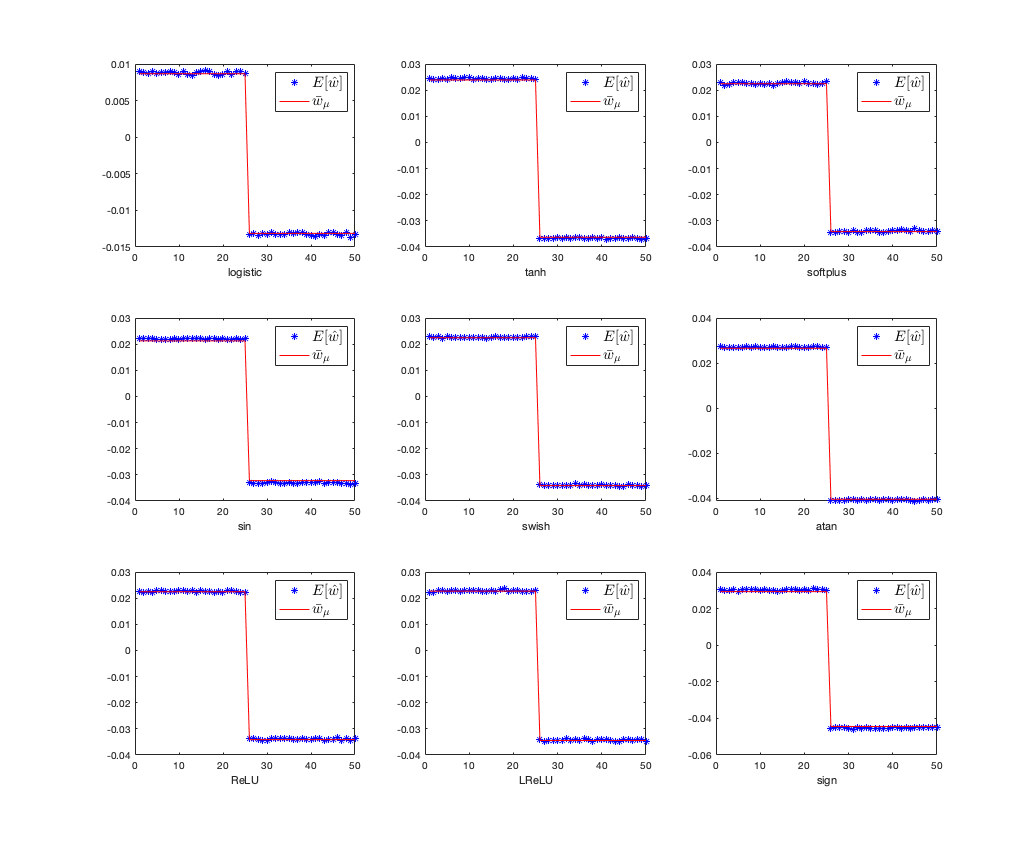
\includegraphics[width=1.1\textwidth]{figs/implicit_reg_nonlinear.png}
%%%
\caption{ $\E[\hat \w]$ and versus $\bar \w_\mu$ for different nonlinearities, $d = 50$, $n = 20$, expectation estimated from $50000$ independent runs.}
\end{figure}


\section{Implicit regularization in single-hidden-layer neural network model}

Consider the random feature model of the type $f_{\bbeta}(\x) = \bbeta^\top \phi(\W^\top \x)$ for some nonlinear function $\phi(\cdot): \R \to \R$, random input $\x \in \R^d$, first layer weight matrix $\W \in \R^{d \times p}$, second layer weight $\bbeta \in \R^p$ and noisy output $y = \bbeta_*^\top \phi(\W^\top \x) + \xi$ with independent noise such that $\E[\xi] = 0$ and $\E[\xi^2]$ is finite. Denote
\begin{equation}
  \bphi_i \equiv \phi(\W^\top \x_i) \in \R^p, \quad \bPhi \equiv \phi(\X \W) \in \R^{n \times p}
\end{equation}
and focus on the set of $\bbeta \in \R^p$ that interpolates the training set $\{\x_i, y_i\}_{i=1}^n$ so that $f_{\bbeta}(\x_i) = y_i$ and select the minimum Euclidean norm solution from this set that is explicitly given by
\[
  \hat \bbeta \equiv \argmin_{ \bbeta^\top \bphi_i =y_i} \| \bbeta\|^2 = \bPhi^\dagger \y.
\]
As a consequence, we have 
\[
  \E[\hat \bbeta] = \E[\bPhi^\dagger \y] = \E[\bPhi^\dagger \bPhi] \bbeta_*
\]
and
\[
  \bar \bbeta_\mu \equiv \argmin_{\bbeta} \left\{ \E_{(\x,y) \sim \mu} (f_{\bbeta}(\x) - y)^2 + \lambda \| \bbeta \|^2 \right\} = (\K + \lambda \I_p)^{-1} \K \bbeta_*
\]
where we denote 
\begin{equation}\label{eq:def-K}
  \K \equiv \E[\bphi \bphi^\top] = \E[\phi(\W^\top \x) \phi(\x^\top \W)] \in \R^{p \times p}.
\end{equation}

It thus remains to show
\[
  \E_\X[\bPhi^\dagger \bPhi] \equiv \E_\X[\phi(\X \W)^\dagger \phi(\X \W)] \simeq (\K + \lambda \I)^{-1} \K
\]
in an operator norm sense, for $\lambda$ the solution to $n = \tr \K (\K + \lambda \I)^{-1}$. \textbf{Important here! Do not \emph{explicitly} depend on the data dimension $d$!}

\begin{lemma}[Concentration of quadratic forms, {\cite[Lemma~1]{louart2018random}}]
For $\x \in \R^d$ having i.i.d.\@ zero mean, unit variance and $K$-sub-Gaussian entries with sub-Gaussian norm $\| [\x]_i \|_{\psi_2} \le K$ and $\A \in \R^{p \times p}$ such that $\| \A \| \le 1$, then, define the random vector $\bphi \equiv \phi(\W^\top \x) \in \R^p$ for $\W \in \R^{d \times p}$ and Lipschitz continuous $\phi(\cdot)$ with parameter $\gamma_\phi$, we have
\[
  \Pr \left\{ \left| \frac1p \bphi^\top \A \bphi - \frac1p \tr \A \K \right| \ge t \right\} \le C e^{- \frac{c p}{ \| \W \|^2 K^2 \gamma_\phi^2 } \min \left( \frac{t^2}{t_0^2}, t \right) }
\]
for $t_0 \equiv |\phi(0)| + \gamma_\rho K \| \W \| \sqrt{ \frac{d}{p} }$ and $\K \in \R^{p \times p}$ defined in \eqref{eq:def-K}.
\end{lemma}

\subsection{Explicit form of \texorpdfstring{$\K$}{K} for Gaussian data}

For standard Gaussian $\x \sim \mathcal N(0,\I_d)$, the matrix $\K(\W)$ defined in \eqref{eq:def-K} involves the $d$-dimensional integration of
\begin{align*}
  \K_{ij} &= \E_\x[\phi(\w_i^\top \x) \phi(\x^\top \w_j)] = (2\pi)^{-\frac{d}2} \int_{\mathbb{R}^d} \phi(\x^\top \w_i) \phi(\x^\top \w_j) e^{-\frac12 \|\x\|^2} d\,\x \\ 
  %%
  &= \frac1{2\pi} \int_{\mathbb{R}} \int_{\mathbb{R}} \sigma(\tilde x_1 \tilde w_{i,1}) \sigma(\tilde x_1 \tilde w_{j,1} + \tilde x_2 \tilde w_{j,2}) e^{-\frac12 (\tilde x_1^2 + \tilde x_2^2) } d\,\tilde x_1 d\,\tilde x_2 \\
  %%%
  &= \frac1{2\pi} \int_{\mathbb{R}^2} \sigma(\tilde \x^\top \tilde \w_i) \sigma(\tilde \x^\top \tilde \w_j) e^{-\frac12 \|\tilde \x\|^2} d\,\tilde \x
\end{align*}
where we applied the Gram-Schmidt process (by first assuming that $\w_i$ and $\w_j$ are linearly independent) and denote $\tilde w_{i,1} = \|\w_i\|$, $\tilde w_{j,1} = \frac{\w_i^\top \w_j}{\|\w_i\|}$, $\tilde w_{j,2} = \|\w_j\| \sqrt{ 1 - \frac{(\w_i^\top \w_j)^2}{ \|\w_i\|^2 \|\w_j\|^2 } }$ as well as $\tilde \x = [\tilde x_1, \tilde x_2]^\top$, $\tilde \w_i = [\tilde w_{i,1},0]^\top$ and $\tilde \w_j = [\tilde w_{j,1},\tilde w_{j,2}]^\top$. As an example, for $\phi(t) = \max(t,0) \equiv \ReLU(t)$, this further simplifies as
\begin{align*}
  \K_{i,j} = \frac1{2\pi} \int_{ \min(\tilde \x^\top \tilde \w_i, \tilde \x^\top \tilde \w_j) \ge 0} \tilde \x^\top \tilde \w_i \cdot \tilde \x^\top \tilde \w_j \cdot e^{-\frac12 \|\tilde \x\|^2} d\,\tilde \x
\end{align*}

With a simple geometric representation we observe 
\[
  \{ \tilde \x~|~\min(\tilde \x^\top \tilde \w_i, \tilde \x^\top \tilde \w_j) \ge 0 \} = \left\{ r \cos(\theta) + r \sin (\theta)~|~r\ge0,~\theta \in \left[ \theta_0 - \frac{\pi}2, \frac{\pi}2 \right] \right\}
\]
with $\theta_0 \equiv \arccos \left( \frac{ \tilde w_{j,1} }{ \|\w_j\| } \right) = \frac{\pi}2 - \arcsin \left( \frac{ \tilde w_{j,1} }{ \|\w_j\| } \right)$. Therefore with a polar coordinate change of variable we deduce, for $\phi(t) = \ReLU(t)$ that
\begin{align*}
  \K_{ij} &= \tilde w_{i,1} \frac1{2\pi} \int_{\theta_0 - \frac{\pi}2}^{\frac{\pi}2} \cos(\theta) \left( \tilde w_{j,1} \cos(\theta) + \tilde w_{j,2} \sin(\theta) \right) d\,\theta \ \int_0^\infty r^3 e^{-\frac12 r^2} d\,r \\
  %%%
  &=\frac1{2\pi} \|\w_i\| \|\w_j\| \left( \sqrt{ 1-\angle(\w_i,\w_j)^2 } + \angle(\w_i,\w_j) \arccos\left( - \angle(\w_i,\w_j) \right) \right)
\end{align*}
with $\angle(\w_i,\w_j) \equiv \frac{\w_i^\top \w_j}{ \|\w_i\| \|\w_j\| }$. More results for various commonly used activations function are given in Table~\ref{tab:K-phi}.

\begin{table*}[t]
\caption{$\K_{ij}$ for different $\phi(\cdot)$, $\angle(\w_i,\w_j) \equiv \frac{\w_i^\top \w_j}{\|\w_i\| \|\w_j\|}$.}
\label{tab:K-phi}
\begin{center}
\begin{tabular}{l|c}
\hline
$\sigma(t)$     & $\K_{ij}$ \\
\hline
$t$    & $\w_i^\top \w_j$\\

$\max(t,0) \equiv \ReLU(t)$     & $\frac1{2\pi} \|\w_i\| \|\w_j\| \left(\angle(\w_i,\w_j)\arccos\left(-\angle(\w_i,\w_j)\right)+\sqrt{1-\angle(\w_i,\w_j)^2}\right)$   \\

$|t|$           & $\frac2\pi \|\w_i\| \|\w_j\| \left(\angle(\w_i,\w_j)\arcsin\left(\angle(\w_i,\w_j)\right)+\sqrt{1-\angle(\w_i,\w_j)^2}\right)$   \\

%$\varsigma_+ \max(t,0)+ \varsigma_- \max(-t,0)$ & $\frac{\|\w_i\| \|\w_j\|}{2\pi} \left[ (\varsigma_+ + \varsigma_-)^2 \sqrt{1 - \angle(\w_i,\w_j)^2 } + \angle(\w_i,\w_j) \left( (\varsigma_+^2 + \varsigma_-^2) \arccos(-\angle(\w_i,\w_j)) - 2\varsigma_+ \varsigma_- \arccos(\angle(\w_i,\w_j)) \right) \right]$\\
$\varsigma_+ \max(t,0)+ \varsigma_- \max(-t,0)$ & $ \frac12 (\varsigma_+^2 + \varsigma_-^2) \w_i^\top\w_j + \frac{\|\w_i\| \|\w_j\|}{2\pi} (\varsigma_+ + \varsigma_-)^2 \left( \sqrt{1 - \angle(\w_i,\w_j)^2 } - \angle(\w_i,\w_j) \arccos(\angle(\w_i,\w_j)) \right) $\\

$1_{t>0}$       & $\frac12 -\frac1{2\pi} \arccos\left(\angle(\w_i,\w_j)\right)$    \\

$\sign(t)$ & $\frac2\pi\arcsin\left(\angle(\w_i,\w_j)\right)$    \\

$\varsigma_2 t^2 + \varsigma_1 t + \varsigma_0$ & $\varsigma_2^2 \left( 2\left( \w_i^\top \w_j \right)^2 + \|\w_i\|^2 \|\w_j\|^2 \right) + \varsigma_1^2 \w_i^\top \w_j + \varsigma_2 \varsigma_0 \left( \|\w_i\|^2 + \|\w_j\|^2 \right) + \varsigma_0^2$\\

$\cos(t)$       & $\exp\left(-\frac12 \left(\|\w_i\|^2 + \|\w_j\|^2\right)\right) \cosh(\w_i^\top \w_j)$  \\

$\sin(t)$       & $\exp\left(-\frac12 \left(\|\w_i\|^2 + \|\w_j\|^2\right)\right) \sinh(\w_i^\top \w_j)$  \\

$\erf(t)$  & $\frac2\pi \arcsin\left(\frac{2\w_i^\top \w_j}{\sqrt{(1+2\|\w_i\|^2)(1+2\|\w_j\|^2)}}\right)$    \\
$\exp(-\frac{t^2}2)$ & $\frac1{ \sqrt{ (1+\|\w_i\|^2) (1+\|\w_j\|^2) - (\w_i^\top \w_j)^2 } }$\\
\hline
\end{tabular}
\end{center}
\end{table*}

\subsection{Simulations}

Questions: 
\begin{enumerate}
  \item condition on the dimensions $n,p,d$?
  \item condition on the weight matrix $\W \in \R^{n \times d}$, should depend on the operator norm of $\W$, is there any dependence on the minimum singular value?
  \item dependence on the nonlinear function $\phi(\cdot)$? should be assumed to be at least Lipschitz (and the results should depend on the Lipschitz constant of $\phi$), but what's the impact of different nonlinearity? Note that the expression of $\K(\W)$ can be given explicitly for some commonly used activation function $\phi$ such as ReLU, etc.
  \item can we go beyond the case of i.i.d.~Gaussian $\X$? should be able to extend to i.i.d.~sub-Gaussian entries, in that case however, the expression of $\K(\W)$ may no longer be explicit.
\end{enumerate}

\clearpage

Consider the random feature model of the type $f_{\bbeta}(\x) = \bbeta^\top \phi(\W^\top \x)$ for some nonlinear function $\phi(\cdot): \R \to \R$, \emph{deterministic} $\x \in \R^d$, $\W \in \R^{d \times p}$ having i.i.d.~Gaussian entries and $\bbeta \in \R^p$ and noisy output $y =  \bbeta_*^\top \phi(\W^\top \x) + \xi$ with independent noise such that $\E[\xi] = 0$ and $\E[\xi^2]$ is finite. Denote
\begin{equation}
  \bphi_i \equiv \phi(\W^\top \x_i) \in \R^p, \quad \bPhi \equiv \phi(\X \W) \in \R^{n \times p}
\end{equation}
and focus on the set of $\bbeta \in \R^p$ that interpolates the training set $\{\x_i, y_i\}_{i=1}^n$ so that $f_{\bbeta}(\x_i) = y_i$ and select the minimum Euclidean norm solution from this set that is explicitly given by
\[
  \hat \bbeta \equiv \argmin_{f_{\bbeta}(\x_i) =y_i} \| \bbeta\|^2 = \bPhi^\dagger \y.
\]
As a consequence, we have 
\[
  \E[\hat \bbeta] = \E[\bPhi^\dagger \y] = \E[\bPhi^\dagger \bPhi] \bbeta_*
\]
and
\[
  \bar \bbeta_\mu \equiv \argmin_{\bbeta} \left\{ \E_{(\x,y) \sim \mu} (f_{\bbeta}(\x) - y)^2 + \lambda \| \bbeta \|^2 \right\} = (\K + \lambda \I_p)^{-1} \K \bbeta_*
\]
where we denote 
\begin{equation}
  \K \equiv \E[\bphi \bphi^\top] = \E_\W[\phi(\W^\top \x) \phi(\x^\top \W)] \in \R^{p \times p}.
\end{equation}

It thus remains to show
\[
  \E_\W[\bPhi^\dagger \bPhi] \equiv \E_\W[\phi(\X \W)^\dagger \phi(\X \W)] \simeq (\K + \lambda \I)^{-1} \K
\]
in an operator norm sense, for $\lambda$ the solution to $n = \tr \K (\K + \lambda \I)^{-1}$.

Consider the particular case of logistic regression, we have 
\[
  \Pr(y_i = 1 \mid \x_i) = \sigma(\w_*^\top \x_i) = 1 - \Pr(y_i = -1 \mid \x_i), \quad \sigma(t) = \frac1{1 + e^{-t}}.
\]
The associated maximum likelihood estimate is given by 
\[
  \argmin_\w \ell(y_i \x_i^\top \w) = , \quad \ell(t) = \ln(1 + e^{-t}).
\]

The idea is to evaluate the implicit ``regularization'' effect. For the minimum norm solution, it thus remains to assess
\begin{equation}\label{eq:implicit-regularization}
  \E[ \X^\dagger \y] = \begin{cases} (\Sigmab + \lambda \I_d)^{-1} \E[y(\x) \x], \quad n < d \\ \Sigmab^{-1} \E[y(\x) \x], \quad n \ge d \end{cases}
\end{equation}
with $\lambda$ the unique solution to $n = \tr \Sigmab (\Sigmab+ \lambda \I_d)^{-1}$.

Consider the nonlinear model $\y = \sigma(\X \w) + \xi$, with $\y \in \mathbb R^n$, $\w \in \mathbb R^d$, $\X \in \mathbb R^{n \times d}$ and independent noise $\xi$ of zero mean. Here $\sigma: \mathbb R \mapsto \mathbb R$ is the \emph{link function}, popular choices of $\sigma(\cdot)$ are
\begin{enumerate}
  \item \emph{logit link function}: $\sigma(t) = \frac1{ 1 + e^{-t} }$;
  \item \emph{prohibit link function}: $\sigma(t) = \Phi(t)$ with $\Phi$ the cumulative distribution function of standard normal;
  \item \emph{cloglog link function}: $\sigma(t) = 1 - e^{-e^t}$;
  \item possible non-differentiable function such as the ReLU $\sigma(t) = \max(t,0)$ in a neural network context.
\end{enumerate}


\begin{theorem}\label{t:main}
Let $f_\theta(x)=x^\top\theta$ and $(x,y)\sim\mu$
  be s.t.~$x\sim\Nc(0,\Sigmab)$ and $y=x^\top\theta^*+\xi$,
  with $\E[\xi]=0$. Assume that $\Sigmab$ has nuclear rank
  $r>2n$. Then, for $g(x)=\|x\|_2^2$ 
  and $\ell(\yh,y)=(\yh-y)^2$, we have:
  \begin{align*}
    \E_{\Dc\sim\mu^n}\big[\theta_\Dc^*(g)\big]
   \ \overset{\epsilon}{\simeq}\ \theta_\mu^*(\ell, \lambda g)
\quad    \text{with}\quad\epsilon = O\big(\tfrac{\sqrt n}r\big),
  \end{align*}
  where $\theta'\overset\epsilon\simeq\theta$ iff
  $\|\theta'-\theta\|_2\leq \epsilon\,\|\theta\|_2$, and we define
  $\lambda$ so that $n=\tr\,\Sigmab(\Sigmab+\lambda\I)^{-1}$.
\end{theorem}
Possible extensions of Theorem \ref{t:main} which we can expect to
obtain:
\begin{enumerate}
\item General Euclidean norms of the form $g(x) = x^\top\A x$,
\item General distribution of $y$, i.e., without the underlying
  $x^\top\theta^*+\xi$ model, 
\item Non-Gaussian distribution of $x$, which might include the random
  features model. 
\end{enumerate}

% \begin{align}
%   \E\Big[\argmin_{\w:\,\X\w=\y}g(\w)\Big]\ \simeq\ \argmin_{\w\in\R^d}\Big\{
%   \E_\mu\big[l(\x^\top\w,y)\big] + \lambda \,g(\w)\Big\},\label{eq:hypothesis}
% \end{align}
% We are motivated by the
% theoretical and empirical results of \cite{surrogate-design} in one
% particular case where the input distribution $\mu_\x$ is Gaussian,
% function $g(\w)$ is the squared $\ell_2$-norm $\|\w\|_2^2$ and
% $l(\yh,y)$ is the square loss $(\yh-y)^2$, which suggest that
% \eqref{eq:hypothesis} is an accurate characterization of implicit
% regularization for a minimum $\ell_2$-norm estimator.  In this case,
% the estimator is given via the Moore-Penrose pseudoinverse,
% $\wbh=\X^\dagger\y$, whereas the right hand side of
% \eqref{eq:hypothesis} is the ridge-regularized least squares
% solution. The characterization is only exact when the random design
% distribution $\X\sim\mu^n$ of the data is appropriately \emph{rescaled}, obtaining a
% \emph{surrogate design} distribution $\Xb\sim S_\mu^n$. However,
% the theoretical characterization derived under the
% surrogate design remains remarkably accurate under the unrescaled
% Gaussian random design. Is the squared $\ell_2$-norm the only choice
% for function $g(\cdot)$ that  yields the explicit
% characterization of implicit regularization? In our first result, we show that the result
% of \cite{surrogate-design} can be extended to all Mahalanobis norms of
% the form $\|\w\|_\A^2=\w^\top\A\w$ (where the $\ell_2$-norm is
% recovered by setting $\A$ to identity), suggesting that the observed phenomenon is more general.
% To establish the result, we have to extend the definition of a
% surrogate design, taking into account the matrix $\A$.
\begin{figure}[H]
\centering
\begin{subfigure}[t]{0.48\textwidth}
%  \begin{center}
    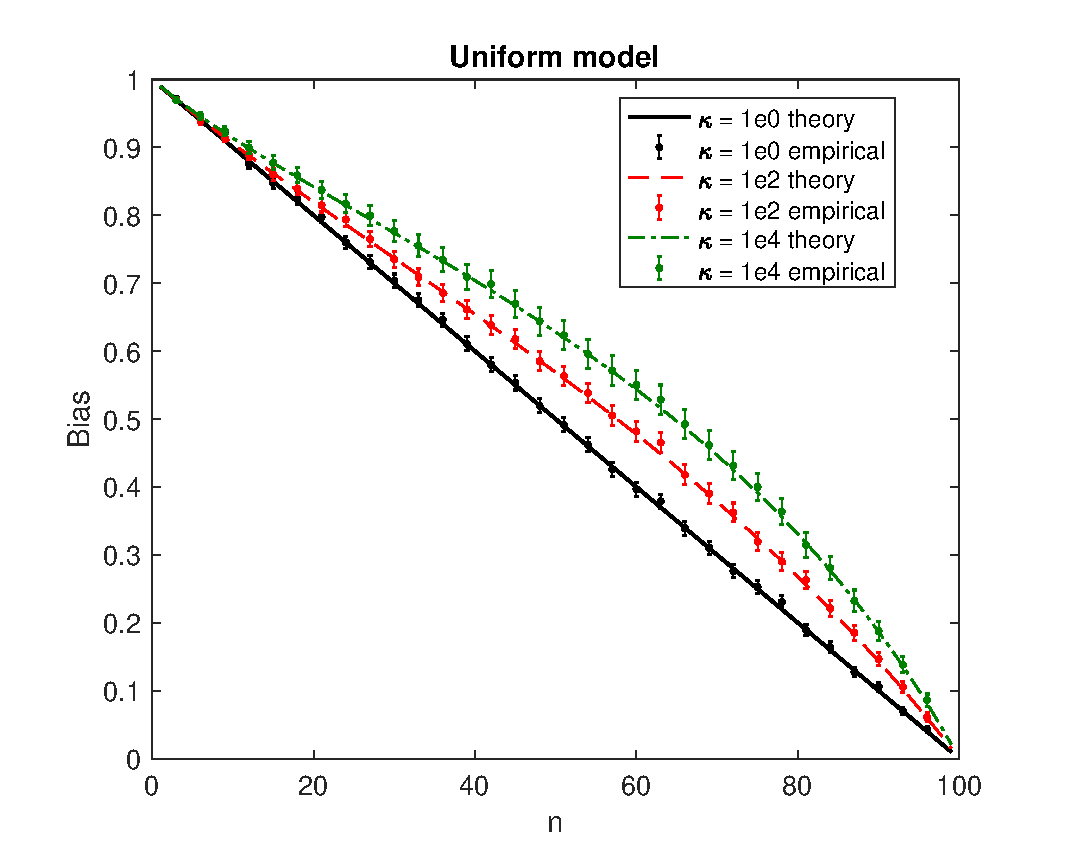
\includegraphics[width=\textwidth]{figs/implicit/implicit_bias_uniform}
%  \end{center}
  \caption{}
\end{subfigure}
\hfill
\begin{subfigure}[t]{0.48\textwidth}
%  \begin{center}
    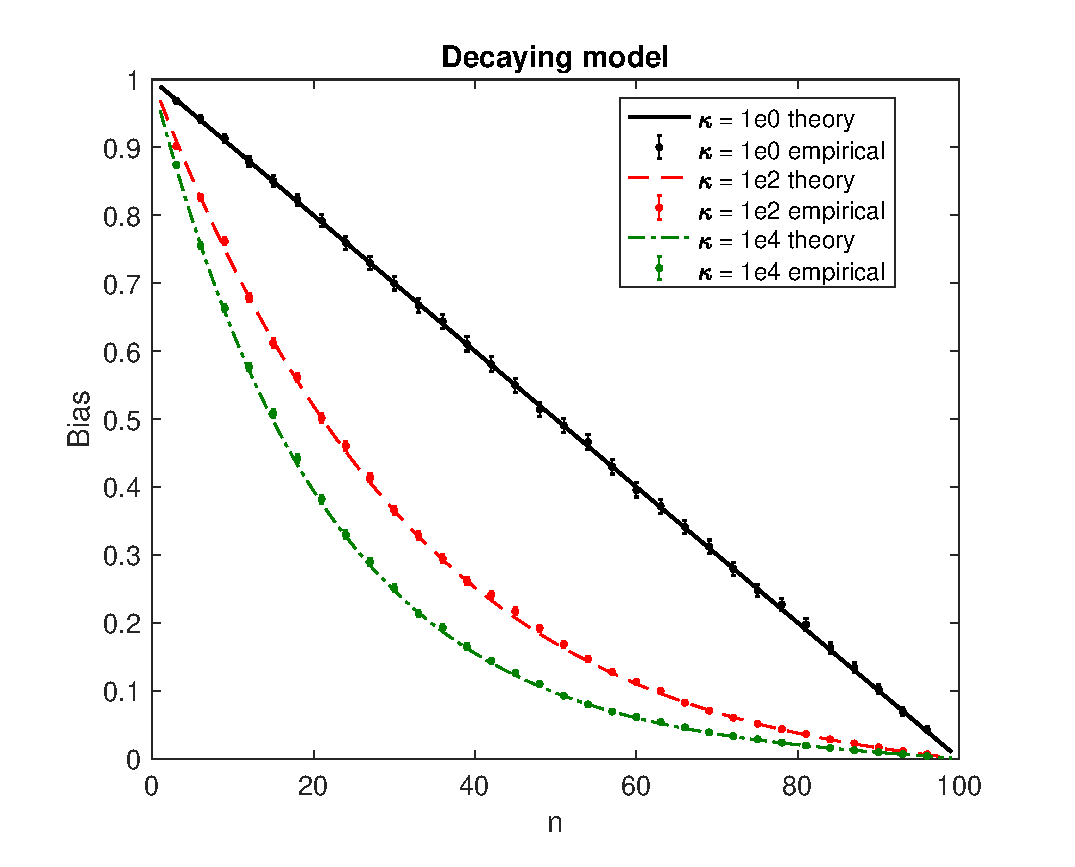
\includegraphics[width=\textwidth]{figs/implicit/implicit_bias_decaying}
%  \end{center}
  \caption{}
\end{subfigure}
\begin{subfigure}[t]{0.48\textwidth}
%  \begin{center}
    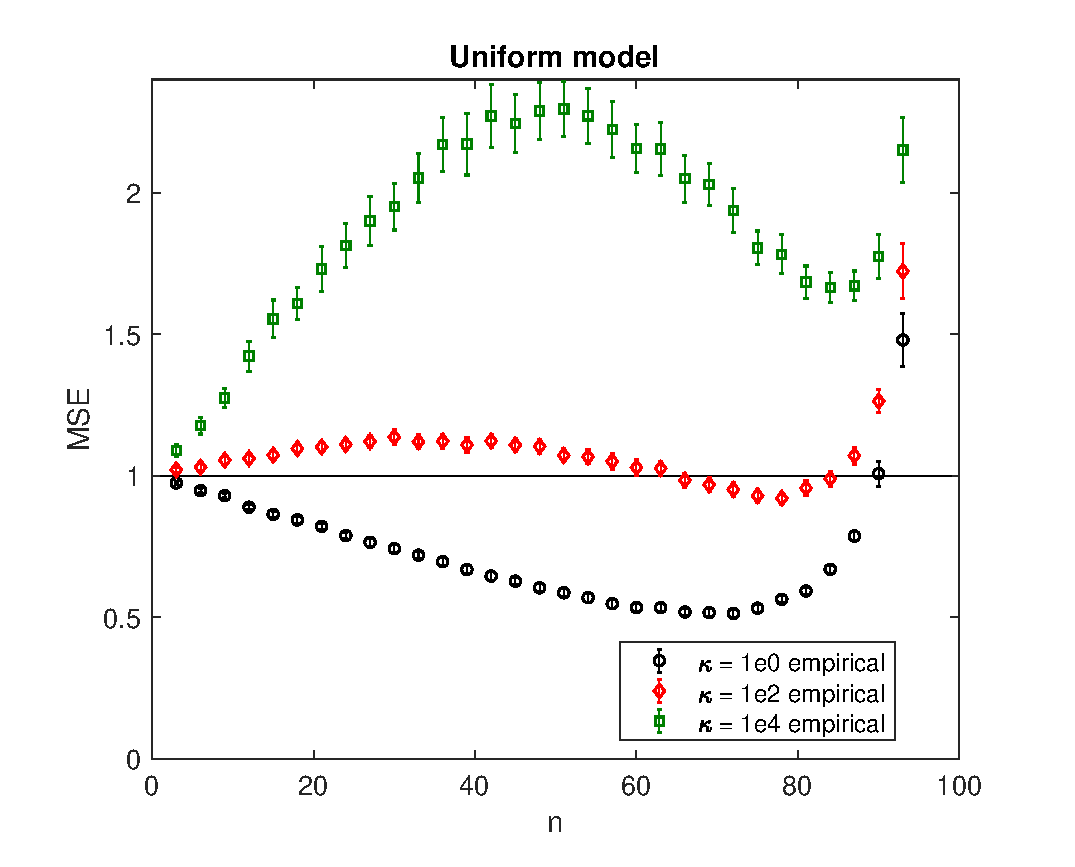
\includegraphics[width=\textwidth]{figs/implicit/implicit_mse_uniform}
%  \end{center}
  \caption{}
\end{subfigure}
\hfill
\begin{subfigure}[t]{0.48\textwidth}
%  \begin{center}
    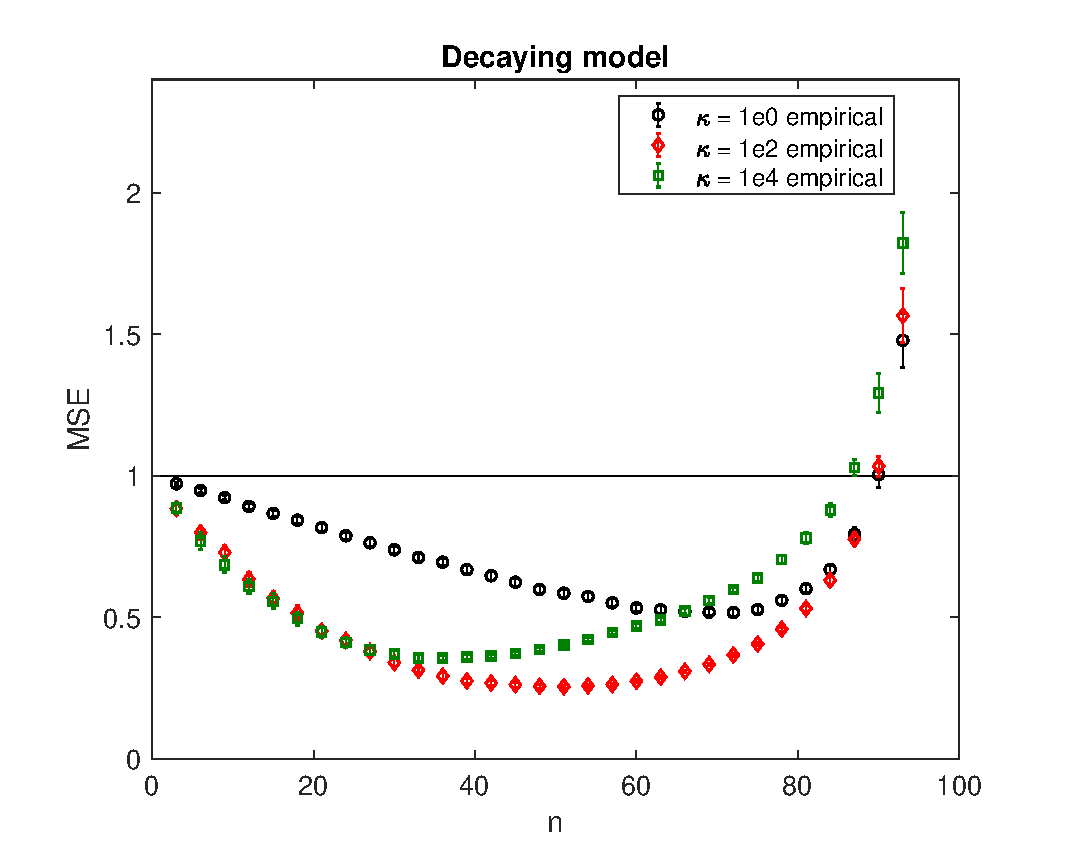
\includegraphics[width=\textwidth]{figs/implicit/implicit_mse_decaying}
%  \end{center}
  \caption{}
\end{subfigure}
\caption{Illustration of using minimum norm estimators for three
  different Mahalanobis norms $\|\cdot\|_A$, with $d=100$ and
  $\mu=\Nc(\zero,\I)$. We consider three matrices $\A$ which are diagonal with
eigenvalues decaying exponentially with condition numbers
$\kappa$. Plots (a) and (b) show the bias, i.e., $\|\E[\wbh]-\w^*\|$,
while plots (c) and (d) show the MSE, i.e.,
$\E\big[\|\wbh-\w^*\|^2\big]$. All plots assume a linear model
$y(\x)=\x^\top\w^*+\xi$, where $\xi\sim \Nc(0,0.3)$. The plots on the
left use a  uniformly linear model, i.e., $\w^*=\frac1{\sqrt{d}}\one$,
whereas the plots on the right use weights increasing exponentially
between  1 and 100, then scaled so that $\|\w^*\|=1$.}
\label{f:intro}
\end{figure}

% \begin{theorem}
%   For any positive definite $\A$,  if $\Xb \sim S_{\!\A,\mu}^n$ then:
%   \begin{align*}
%     \E\Big[\argmin_{\w:\,\Xb\w=\ybb}\|\w\|_\A^2\Big] \ = \
%     \argmin_{\w\in\R^d}\Big\{
%   \E_\mu\big[(\x^\top\w-y)^2\big] + \lambda_n\|\w\|_\A^2\Big\},
%   \end{align*}
%   where $\lambda_n$ is such that
%   $n=\tr\big(\Sigmab_\mu(\Sigmab_\mu+\lambda_n\A)^{-1}\big)$ and
%   $\Sigmab_\mu=\E_\mu[\x\x^\top]$.
% \end{theorem}
% Observe that our surrogate design $S_{\!\A,\mu}^n$ depends on the
% choice of matrix $\A$ even though the original design $\mu^n$ does
% not. Nevertheless, our empirical results (Figure \ref{f:intro}) suggest that under very mild
% assumptions on $\A$, any surrogate design $S_{\!\A,\mu}^n$ closely
% preserves the properties of the original design.

\begin{enumerate}
  \item Can we empirically show \eqref{eq:hypothesis} for
    non-Euclidean norms, where the minimum-norm estimator does not
    have a closed form expression, such as the $\ell_1$-norm?
  \item If the data distribution is not Gaussian, can we replace the
    square loss  $\l(\yh,y)=(\yh-y)^2$ with some other loss to improve
    the accuracy of the characterization?
\end{enumerate}

\section*{Connections to Fenchel duality}

For a convex function $g : \mathbb{R}^d \to \mathbb{R}$, denote its convex
conjugate $g^*(z) = \sup_x z^\top x - f(x) = -\inf f(x) - z^\top x$. We have
\begin{align*}
  \min_{\w : \X \w = \y} g(\w)
  &= \min_{\w \in \mathbb{R}^d} \max_{\v \in \mathbb{R}^n} g(\w) + \v^\top (\y - \X \w) \\
  &\geq \max_{\v \in \mathbb{R}^n} \min_{\w \in \mathbb{R}^d} g(\w) + \v^\top (\y - \X \w) \\
  &= \max_{\v \in \mathbb{R}^n} \v^\top \y - g^*(\X^\top \v)
\end{align*}
with the inequality an equality under certain conditions (Sion minimax theorem).
Assume equality for what remains.

From first order conditions, the optimal $\v$ satisfies
\begin{align*}
  \y &= \X (\nabla g^*)(\X^\top \v)
\end{align*}
For example, when $g(\z) = \frac{1}{2} \z^\top \z$ then $g = g^*$, $\nabla g^*(\z) = \z$,
and we have $\y = \X \X^\top \v$ hence $\v = (\X \X^\top)^{-1} \y$ and
\begin{align*}
  \max_{\v \in \mathbb{R}^n} \min_{\w \in \mathbb{R}^d} g(\w) + \v^\top (\y - \X \w)
  &= \min_{\w \in \mathbb{R}^d} g(\w) + \y^\top (\X \X^\top)^{-1} (\y - \X \w) \\
  &= \min_{\w \in \mathbb{R}^d} \|\y - \X \w\|_2^2 + g(\w) + \left(\y^\top (\X \X^\top)^{-1} - (\y - \X \w)^\top\right) (\y - \X \w) \\
  &= \min_{\w \in \mathbb{R}^d} \|\y - \X \w\|_2^2 + g(\w) + \left(
    \y^\top ((\X \X^\top)^{-1} - \I) + \w^\top \X^\top
  \right) (\y - \X \w)
\end{align*}
Optimizing over $\w$ only involves retaining terms containing $\w$ so
ignoring constants and focusing on those terms shows
\begin{align*}
  \min_{\w : \X \w = \y} g(\w)
  &= \min_{\w \in \mathbb{R}^d} \|\y - \X \w\|_2^2 + g(\w)
    - \y^\top ((\X \X^\top)^{-1} - \I) \X \w + \w^\top \X^\top \y - \w^\top \X^\top \X \w \\
  &= \min_{\w \in \mathbb{R}^d} \|\y - \X \w\|_2^2 + g(\w)
    + \y^\top (2 \I - (\X \X^\top)^{-1}) \X \w
    - \w^\top \X^\top \X \w
\end{align*}
Assume a linear $y(\x) = \x^\top \w^* + \xi$ model and take expectation,
using Fatou's lemma to move the expectation into the minimization
\begin{align*}
  \E \min_{\w \in \mathbb{R}^d} (\cdot)
  &\leq \min_{\w \in \mathbb{R}^d} \E\left[
    \|\y - \X \w\|_2^2 + g(\w)
    + \y^\top (2 \I - (\X \X^\top)^{-1}) \X \w
    - \w^\top \X^\top \X \w
  \right] \\
  &= \min_{\w \in \mathbb{R}^d} \E\left[
    \|\y - \X \w\|_2^2
    + \w^\top \X^\top (\I - (\X \X^\top)^{-1}) \X \w
  \right]
  + g(\w) \\
  &= \min_{\w \in \mathbb{R}^d} \E\left[
    \|\y - \X \w\|_2^2
    + \w^\top (\X^\top \X - \X^\dag \X) \w
  \right]
  + g(\w)
\end{align*}
Approximating $\E[\X^\top \X - \X^\dag \X] \approx \lambda \I$ and
recalling $g(\w) = \frac{1}{2} \w^\top \w$, we have
\begin{align*}
  \E \min_{\w \in \mathbb{R}^d} (\cdot)
  &\leq \min_{\w \in \mathbb{R}^d} \E\left[
    \|\y - \X \w\|_2^2
  \right]
  + \left(\lambda + 1\right)g(\w)
\end{align*}

\bibliographystyle{alpha}
\bibliography{pap}


\end{document}
